%=================================================================
% This template is based on IMRT Latex template by Eric A. Mueller
%================================================================= 

\documentclass[10pt,twoside,a4paper]{report}

 \usepackage[mt,hs,english]{styles/ethasl}   % New styles and commands
                                      % Options:
                                      % bt/mt: Bachelorthesis/Masterthesis
                                      % fs/hs: Frühlingssemester/Herbstsemester
                                      % german/english: Deutsch/English

% \includeonly{}                      % Quick formatting
% \usepackage[draft]{graphicx}        % Quick formatting

 \usepackage{a4}                      % Paper size
 \usepackage[utf8]{inputenc}          % Keyboard settings
 \usepackage{amsmath}                 % Additional math functionality
 \usepackage{amssymb}                 % Additional math functionality
 \usepackage{graphicx}                % EPS figures
 \usepackage[dvips]{epsfig}           % EPS figures
 \usepackage{float}                   % Placement of floating objects
 \usepackage{fancyhdr}                % Headings
 \usepackage{rotating}
 \usepackage{multirow}
 \usepackage{url}
 \usepackage{colortbl}
 \usepackage{ifpdf}
 \usepackage{hyperref}
 \usepackage{upgreek}
 \usepackage{nicefrac}
 \usepackage{units}
 \usepackage{color}
 
 \definecolor{black}{rgb}{0,0,0}
 \definecolor{white}{rgb}{1,1,1}
 \definecolor{darkred}{rgb}{0.5,0,0}
 \definecolor{darkgreen}{rgb}{0,0.5,0}
 \definecolor{darkblue}{rgb}{0,0,0.5}

 \hypersetup{colorlinks
	,linkcolor=black
	,filecolor=black
	,urlcolor=black
	,citecolor=black
 }
 
 % ISO math notation
 \usepackage{isomath}
 \renewcommand{\vec}{\vectorsym}
 \newcommand{\mat}{\matrixsym}
 
 % Left exp and sup
 \newcommand{\leftexp}[2]{{\vphantom{#2}}^{#1}{#2}}
 \newcommand{\leftsub}[2]{{\vphantom{#2}}_{#1}{#2}}

 \ifpdf
	\usepackage[update]{epstopdf}
 \else
 \fi

% \usepackage{german}                  % German language
% \usepackage{ae}                      % German specials

%---------------------------------------------------------------------------

 \setlength{\parindent}{0em}                   % Disable parindent
 \rhead[\thepage]{\nouppercase{\rightmark}}    % Special headings
 \lhead[\nouppercase{\leftmark}]{\thepage}     % Special headings
 \cfoot{}                                      % Special headings

%---------------------------------------------------------------------------

 \title{\LaTeX\ \!-Template für Semester- und Diplomarbeiten}
 %\subtitle{bla bla bla}

 \studentA{Student 1}
 \studentB{Student 2}
% \studentC{Student 3}

\supervisionA{Andreas Muster}
%\supervisionB{Supervisor B}
%\supervisionC{Supervisor C}
 

%===========================================================================
\begin{document}

%---------------------------------------------------------------------------
% Title page

 \maketitle
 \pagestyle{plain}
 \pagenumbering{roman}

%---------------------------------------------------------------------------
% Declaration of Originality

\pagestyle{empty}
% TODO Modify placeholders in declaration.tex
% TODO Add title, student first/last name, supervisor first/last name.

\section*{Declaration of Originality}

\vspace{1cm}

I hereby declare that the written work I have submitted entitled

\vspace{0.5cm}

% TODO Add title
\textbf{Your Project Title}

\vspace{0.5cm}

is original work which I alone have authored and which is written in my own words.\footnote{Co-authored work: The signatures of all authors are required. Each signature attests to the originality of the entire piece of written work in its final form.}

\vspace{1cm}

\textbf{Author(s)}

\vspace{0.5cm}

\begin{tabular}{ p{5cm} p{5cm} }
% TODO Add student first/last name
  First name & Last name \\
\end{tabular}

\vspace{0.5cm}

\textbf{Student supervisor(s)}

\vspace{0.5cm}

\begin{tabular}{ p{5cm} p{5cm} }
% TODO Add supervisor first/last name
  First name & Last name \\
\end{tabular}

\vspace{0.5cm}

\textbf{Supervising lecturer}

\vspace{0.5cm}

\begin{tabular}{ p{5cm} p{5cm} }
  Roland & Siegwart \\
\end{tabular}

\vspace{1cm}

With the signature I declare that I have been informed regarding normal academic citation rules and that I have read and understood the information on 'Citation etiquette' (\url{https://www.ethz.ch/content/dam/ethz/main/education/rechtliches-abschluesse/leistungskontrollen/plagiarism-citationetiquette.pdf}).
The citation conventions usual to the discipline in question here have been respected.

\vspace{0.5cm}

The above written work may be tested electronically for plagiarism.

\vspace{4cm}

\begin{tabular}{ p{5cm} p{1cm} p{5cm} }
  \cline{1-1} \cline{3-3}
  Place and date & & Signature \\
\end{tabular}


%---------------------------------------------------------------------------
% Preamble

 %---------------------------------------------------------------------------
% Preface

%\chapter*{Vorwort}

%Bla bla \dots

 %\cleardoublepage

%---------------------------------------------------------------------------
% Table of contents

 \setcounter{tocdepth}{2}
 \tableofcontents

 \cleardoublepage

%---------------------------------------------------------------------------
% Abstract

%\chapter*{Zusammenfassung}
% \addcontentsline{toc}{chapter}{Zusammenfassung}

%Bla bla \dots

% \cleardoublepage

\chapter*{Abstract}
 \addcontentsline{toc}{chapter}{Abstract}

Hier kommt der Abstact hin \dots

 \cleardoublepage

%---------------------------------------------------------------------------
% Symbols

%\chapter*{Symbolverzeichnis}\label{chap:symbole}
% \addcontentsline{toc}{chapter}{Symbolverzeichnis}
\chapter*{Symbols}\label{chap:symbole}
 \addcontentsline{toc}{chapter}{Symbols}

%\section*{Symbole}
\section*{Symbols}
\begin{tabbing}
 \hspace*{3cm} \= \kill
  $\phi, \theta, \psi$ 					\> roll, pitch and yaw angle \\[0.5ex] 					
  $b$														\> gyroscope bias \\[0.5ex]										
  $\Omega_m$										\> 3-axis gyroscope measurement \\[0.5ex]   		
 \end{tabbing}

%\section*{Indizes}
\section*{Indices}
\begin{tabbing}
 \hspace*{1.6cm}  \= \kill
 $x$ \> x axis \\[0.5ex]
 $y$ \> y axis \\[0.5ex]
 
\end{tabbing}

%\section*{Akronyme und Abkürzungen}
\section*{Acronyms and Abbreviations}
\begin{tabbing}
 \hspace*{1.6cm}  \= \kill
 ETH \> Eidgenössische Technische Hochschule \\[0.5ex]
 EKF \> Extended Kalman Filter \\[0.5ex]
 IMU \> Inertial Measurement Unit \\[0.5ex]
 UAV \> Unmanned Aerial Vehicle \\[0.5ex]
 UKF \> Unscented Kalman Filter \\[0.5ex]
\end{tabbing}

 \cleardoublepage

%---------------------------------------------------------------------------


 \pagestyle{headings}                 % Default headings
 \pagestyle{fancy}                   % Special headings
 \pagenumbering{arabic}

%---------------------------------------------------------------------------
% Chapters

 
%\chapter{Einleitung}\label{sec:einleitung}
\chapter{Introduction}\label{sec:introduction}

Hier kommt die Einleitung
 \cleardoublepage
 \chapter{Einige wichtige Hinweise zum Arbeiten mit \LaTeX\ }
\label{sec:latexumg}

Nachfolgend wird die Codierung einiger oft verwendeten Elemente
kurz beschrieben. Das Einbinden von Bildern ist in \LaTeX\ nicht
ganz unproblematisch und hängt auch stark vom verwendeten Compiler
ab. Typisches Format für Bilder in \LaTeX\ ist
EPS\footnote{Encapsulated Postscript} oder PDF\footnote{Portable Document Format}.


\section{Gliederungen}
\label{sec:gliederung}

Ein Text kann mit den Befehlen \texttt{\textbackslash
chapter\{.\}}, \texttt{\textbackslash section\{.\}},
\texttt{\textbackslash subsection\{.\}} und \texttt{\textbackslash
subsubsection\{.\}} gegliedert werden.


\section{Referenzen und Verweise}
\label{sec:refverw}

Literaturreferenzen werden mit dem Befehl \texttt{\textbackslash
cite\{.\}} erzeugt. Beispiele: ein Buch \cite{Raibert1986LeggedRobotsThatBalance}, ein Buch und ein Journal Paper \cite{Raibert1986LeggedRobotsThatBalance,Vukobratovic2004ZeroMomentPoint}, ein Konferenz Paper mit Erwähnung des Autors: \citet{Pratt1995SEA}.

Zur Erzeugung von Fussnoten wird der Befehl \texttt{\textbackslash
footnote\{.\}} verwendet. Auch hier ein Beispiel\footnote{Bla
bla.}.

Querverweise im Text werden mit \texttt{\textbackslash label\{.\}}
verankert und mit \texttt{\textbackslash ref\{.\}} erzeugt.
Beispiel einer Referenz auf das zweite Kapitel:
Kapitel~\ref{sec:latexumg}.


\section{Aufzählungen}\label{sec:aufz}

Folgendes Beispiel einer Aufzählung ohne Numerierung,
\begin{itemize}
  \item Punkt 1
  \item Punkt 2
\end{itemize}
wurde erzeugt mit:
\begin{verbatim}
\begin{itemize}
  \item Punkt 1
  \item Punkt 2
\end{itemize}
\end{verbatim}

Folgendes Beispiel einer Aufzählung mit Numerierung,
\begin{enumerate}
  \item Punkt 1
  \item Punkt 2
\end{enumerate}
wurde erzeugt mit:
\begin{verbatim}
\begin{enumerate}
  \item Punkt 1
  \item Punkt 2
\end{enumerate}
\end{verbatim}

Folgendes Beispiel einer Auflistung,
\begin{description}
  \item[P1] Punkt 1
  \item[P2] Punkt 2
\end{description}
wurde erzeugt mit:
\begin{verbatim}
\begin{description}
  \item[P1] Punkt 1
  \item[P2] Punkt 2
\end{description}
\end{verbatim}


\section{Erstellen einer Tabelle}\label{sec:tabellen}

Ein Beispiel einer Tabelle:
\begin{table}[h]
\begin{center}
 \caption{Daten der Fahrzyklen ECE, EUDC, NEFZ.}\vspace{1ex}
 \label{tab:tabnefz}
 \begin{tabular}{ll|ccc}
 \hline
 Kennzahl & Einheit & ECE & EUDC & NEFZ \\ \hline \hline
 Dauer & s & 780 & 400 & 1180 \\
 Distanz & km & 4.052 & 6.955 & 11.007 \\
 Durchschnittsgeschwindigkeit & km/h & 18.7 &  62.6 & 33.6 \\
 Leerlaufanteil & \% & 36 & 10 & 27 \\
 \hline
 \end{tabular}
\end{center}
\end{table}

Die Tabelle wurde erzeugt mit:
\begin{verbatim}
\begin{table}[h]
\begin{center}
 \caption{Daten der Fahrzyklen ECE, EUDC, NEFZ.}\vspace{1ex}
 \label{tab:tabnefz}
 \begin{tabular}{ll|ccc}
 \hline
 Kennzahl & Einheit & ECE & EUDC & NEFZ \\ \hline \hline
 Dauer & s & 780 & 400 & 1180 \\
 Distanz & km & 4.052 & 6.955 & 11.007 \\
 Durchschnittsgeschwindigkeit & km/h & 18.7 &  62.6 & 33.6 \\
 Leerlaufanteil & \% & 36 & 10 & 27 \\
 \hline
 \end{tabular}
\end{center}
\end{table}
\end{verbatim}


\section{Einbinden einer Grafik}\label{sec:epsgraph}

Das Einbinden von Graphiken kann wie folgt bewerkstelligt werden:
\begin{verbatim}
\begin{figure}
   \centering
   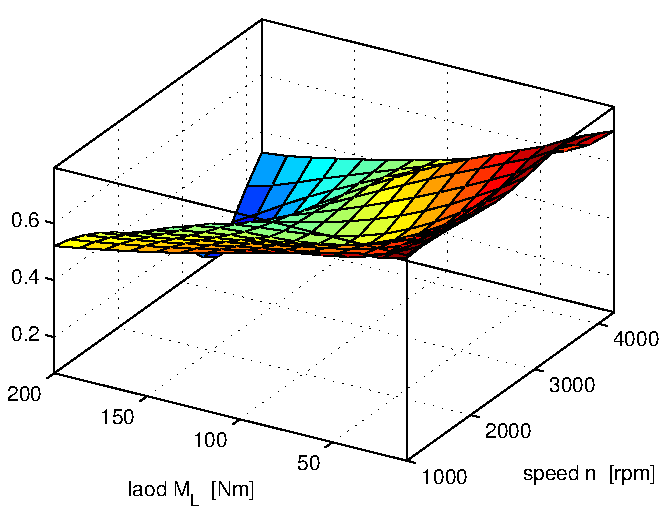
\includegraphics[width=0.75\textwidth]{images/k_surf.pdf}
   \caption{Ein Bild.}
   \label{fig:k_surf}
\end{figure}
\end{verbatim}

\begin{figure}
   \centering
   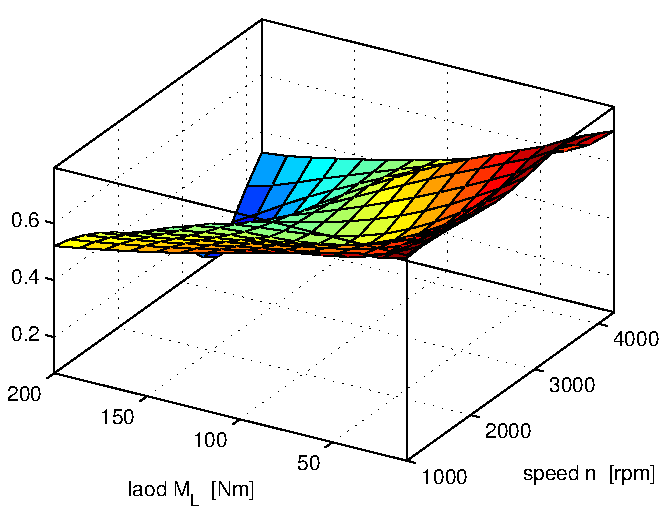
\includegraphics[width=0.75\textwidth]{images/k_surf.pdf}
   \caption{Ein Bild}
   \label{pics:k_surf}
\end{figure}

oder bei zwei Bildern nebeneinander mit:
\begin{verbatim}
\begin{figure}
  \begin{minipage}[t]{0.48\textwidth}
    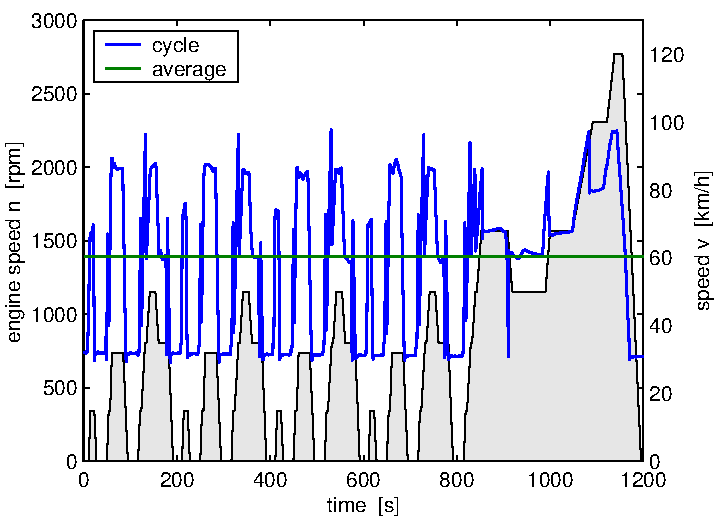
\includegraphics[width = \textwidth]{images/cycle_we.pdf}
  \end{minipage}
  \hfill
  \begin{minipage}[t]{0.48\textwidth}
    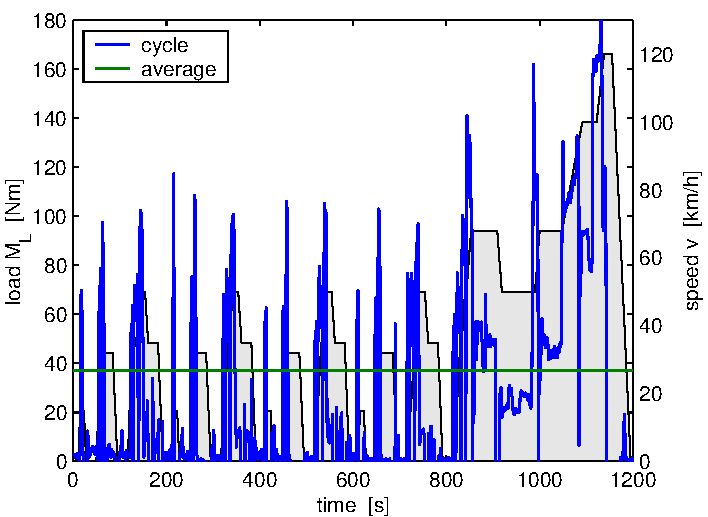
\includegraphics[width = \textwidth]{images/cycle_ml.pdf}
  \end{minipage}
  \caption{Zwei Bilder nebeneinander.}
  \label{pics:cycle}
\end{figure}
\end{verbatim}

\begin{figure}
  \begin{minipage}[t]{0.48\textwidth}
    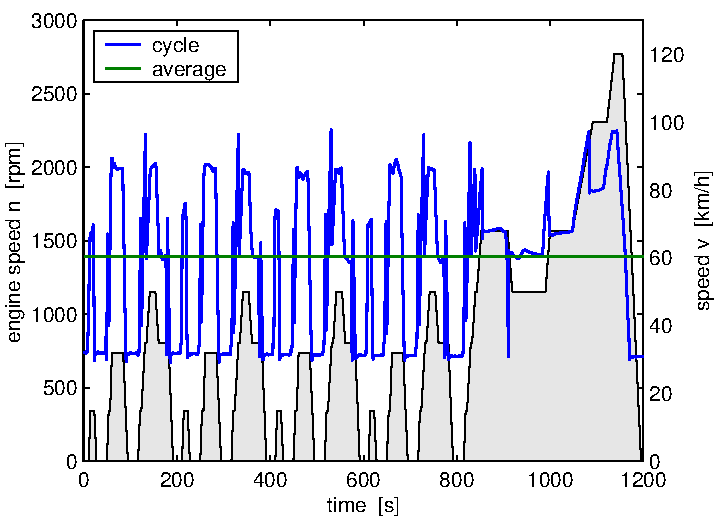
\includegraphics[width = \textwidth]{images/cycle_we.pdf}
  \end{minipage}
  \hfill
  \begin{minipage}[t]{0.48\textwidth}
    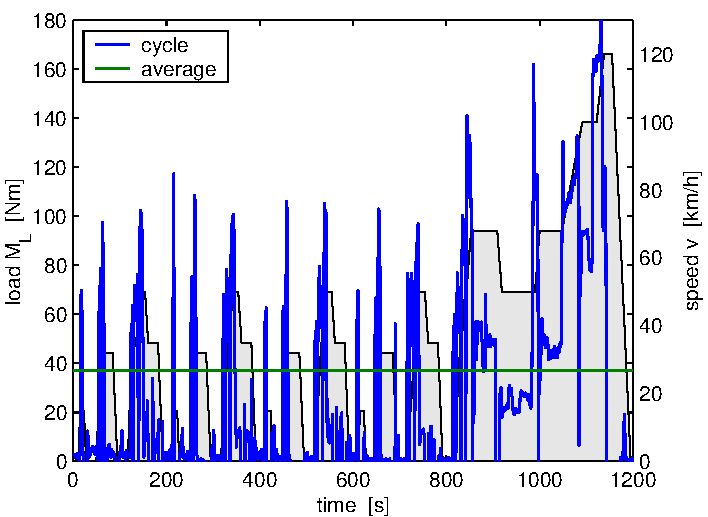
\includegraphics[width = \textwidth]{images/cycle_ml.pdf}
  \end{minipage}
  \caption{Zwei Bilder nebeneinander}
  \label{pics:cycle}
\end{figure}


\section{Mathematische Formeln}\label{sec:math}

Einfache mathematische Formeln werden mit der equation-Umgebung
erzeugt:
\begin{equation}
 p_{me0f}(T_e,\omega_e) \ = \ k_1(T_e) \cdot (k_2+k_3 S^2
 \omega_e^2) \cdot \Pi_{\mathrm{max}} \cdot \sqrt{\frac{k_4}{B}} \, .
\end{equation}

Der Code dazu lautet:
\begin{verbatim}
\begin{equation}
 p_{me0f}(T_e,\omega_e) \ = \ k_1(T_e) \cdot (k_2+k_3 S^2
 \omega_e^2) \cdot \Pi_{max} \cdot \sqrt{\frac{k_4}{B}} \, .
\end{equation}
\end{verbatim}

Mathematische Ausdrücke im Text werden mit \$formel\$ erzeugt (z.B.:
$a^2+b^2=c^2$).

Vektoren und Matrizen werden mit den Befehlen \texttt{\textbackslash vec\{.\}} und \texttt{\textbackslash mat\{.\}} erzeugt (z.B. $\vec{v}$, $\mat{M}$).


\section{Weitere nützliche Befehle}\label{sec:div}

Hervorhebungen im Text sehen so aus: \emph{hervorgehoben}. Erzeugt
werden sie mit dem \texttt{\textbackslash epmh\{.\}} Befehl.

Einheiten werden mit den Befehlen \texttt{\textbackslash unit[1]\{m\}} (z.B.~\unit[1]{m}) und \texttt{\textbackslash unitfrac[1]\{m\}\{s\}} (z.B.~\unitfrac[1]{m}{s}) gesetzt.

 \cleardoublepage
% \include{}
% \cleardoublepage
% \include{}
% \cleardoublepage
% ...
%
%---------------------------------------------------------------------------
% Appendix

 \appendix
 \chapter{Irgendwas}\label{sec:irgendwas}

Bla bla \dots
%
%---------------------------------------------------------------------------
% Literature

 
\begin{thebibliography}{99}
%\addcontentsline{toc}{chapter}{Literaturverzeichnis}
\addcontentsline{toc}{chapter}{Bibliography}



\bibitem {comfilt} {\sc R.~Mahony, T.~Hamel, J.-M.~Pflimlin}:
{\it Complementary filter design on the special orthogonal group SO(3)}. In 45th Conference
on Decision and Control CDC'05, Seville, Spain, 2005.


\end{thebibliography}


%---------------------------------------------------------------------------

\end{document}
%===========================================================================
